
\documentclass[12pt]{article}
\usepackage{amsmath}
\DeclareMathOperator*{\argmin}{arg\,min} % thin space, limits underneath in displays
\DeclareMathOperator*{\argmax}{arg\,max} % thin space, limits underneath in displays
\newtheorem{thm}{Theorem}
\usepackage{amssymb}
\usepackage{amsfonts}
\usepackage{mathrsfs}
\usepackage{bm}
\usepackage{indentfirst}
\setlength{\parindent}{0em}
\usepackage[margin=1in]{geometry}
\usepackage{graphicx}
\usepackage{setspace}
\doublespacing
\usepackage[flushleft]{threeparttable}
\usepackage{booktabs,caption}
\usepackage{float}
\usepackage{graphicx}
\usepackage[sort,comma]{natbib}

\usepackage{import}
\usepackage{xifthen}
\usepackage{pdfpages}
\usepackage{transparent}

\newcommand{\incfig}[1]{%
\def\svgwidth{\columnwidth}
\import{./figures/}{#1.pdf_tex}
}




\title{}
\author{}
\date{}


\begin{document}
\maketitle
\section{Three statistics}
{\textbf {GDP:}}\\
Gross domestic product, or GDP, tells us the nation’s total income and the total 
expenditure on its output of goods and services.

{\textbf {CPI:}}\\
The consumer price index, or CPI, measures the level of prices. 

{\textbf {Unemployment rate:}}\\
The unemployment rate tells us the fraction of workers who are unemployed. 



\subsection{GDP}
There are two ways to view this statistic. 
One way to view GDP is as the total income of everyone in the
economy; another way is as the total expenditure on the economy’s output of goods 
and services. From either viewpoint, it is clear why GDP is a gauge of economic 
performance. How can GDP measure both the economy’s income and its expenditure on output?
It can do so because these two quantities are really the same: for the economy as 
a whole, income must equal expenditure. That fact, in turn, follows from an even more
fundamental one: because every transaction has a buyer and a seller,
every dollar of expenditure by a buyer must become a dollar of income to a seller. 
When Jack paints Jill’s house for \$10,000, that \$10,000 is income to Jack and 
expenditure by Jill. The transaction contributes \$10,000 to GDP, regardless of whether 
we are adding up all income or all expenditure.



\subsubsection{Two ways to compute GDP}

\begin{figure}[H]
\center{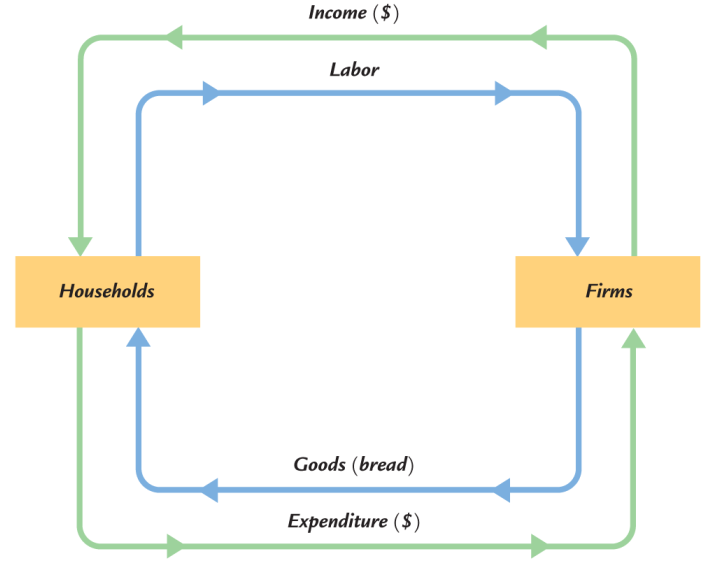
\includegraphics[scale =.5 ]  {figures/income_expenditure_circle_gdp.png}}
\end{figure}
{\textbf {1: Seller}}\\
We can compute it in two ways. GDP is the total income from the production of bread,
which equals the sum of wages and profit — the top half of the circula  flow of dollars.
(wage + profit = firm's income) 

{\textbf {2: Buyer}}\\
GDP is also the total expenditure on purchases of bread — the bottom half of the 
circular flow of dollars. To compute GDP, we can look at either the flow of dollars
from firms to households or the flow of dollars from households to firms.


{\textbf {These two ways of computing GDP must be equal because the expenditure of
buyers on products is income to the sellers of those products.}}


\subsubsection{Rules for computing GDP}
1. Values = price * quantity

2. Transfer is not part of GDP: Firm A produces and sells product for \$2, this is part
of the GDP. But if a collector sell a card to another collector for \$2, this is NOT
part of GDP. It is a transfer of an asset, not an addition to national income.


3. Inventory:\\
When a firm increases its inventory of goods, this investment in inventory is counted as
expenditure by the firm owners. Thus, production for inventory increases GDP just as much
as does production for final sale.

A sale out of inventory, however, combines positive spending (the purchase) and negative
spending (inventory disinvestment), so it does not affect GDP. This treatment of inventor
ies ensures that GDP reflects the economy’s current production of goods and services.


4. Intermediate goods:\\
Suppose a cattle rancher sells one-quarter pound of meat to McDonald’s for \$1, and 
then McDonald’s sells you a hamburger for \$3. 
GDP includes only the value of final goods. Thus, the hamburger is included in GDP, 
but the meat is not: GDP increases by \$3, not by \$4.
The reason is that the value of intermediate goods is already included as part of the 
market price of the final goods in which they are used.

Or we can calculate the value added. \$1 added for meat, and 3-1 = \$2 added for 
hamburger. Hence, total added value = 1+2 = 3.


5. Imputations:\\
Not all goods and services are sold in the mkt. Hence not all products have prices.
For these goods, we need to estimate the imputed value.

{\textbf {Case1: Housing}}\\
Renter pay rents to house owner. There's a expenditure for renter and a income for 
house owner. So this is counted as part of GDP. However, for those who live in their
own house, they also enjoy the service of housing, GDP includes the ``rent" they
pay to themselves. The department of commerce estimates the mkt rent. This imputed
value will be included in both houseowner's expenditure and income.


{\textbf {Case2:Gov't Services}}\\
Police officers, firefighters, and senators provide services to the public, but do not
have market price. The national accounts include these to services using their cost
e.g., the wage.

{\textbf {Not included:}}\\
Rent on cars, lawn mowers, jewelry, and other durable goods owned by households.
Yet the value of these rental services is left out of GDP.

Some of the output of the economy is produced and consumed at home and never enters the 
marketplace. They are out of the GDP, for example, home-made food.

No imputation is made for the value of goods and services sold in the 
{\textbf {underground economy}}.


{\textbf {NOTE:}}\\
Because the imputations necessary for computing GDP are only approximate, and because the value of many goods and services is left out altogether, GDP is an imperfect measure of economic activity.


\subsubsection{Nominal vs. Real GDP}

Economists use real GDP, which is the value of goods and services measured using a 
constant set of prices. That is, real GDP shows what would have happened to
expenditure on output if quantities had changed but prices had not.\\
If we use 2017 as base year, then real GDP in 2018 and 2019 would be:

Real GDP 2018:
\begin{equation*}
\text{ Real GDP }_{2018} = \text{ price }_{2017}  \times \text{ quantity }_{2018}
\end{equation*}


Real GDP 2019:
\begin{equation*}
\text{ Real GDP }_{2019} = \text{ price }_{2017}  \times \text{ quantity }_{2019}
\end{equation*}



\subsubsection{GDP Deflator}
{\textbf {GDP deflator}}, also called {\textbf {implicit price deflator}} for GDP,
is the ratio of nominal GDP to real GDP:

\begin{equation*}
\text{ GDP deflator } = \frac{\text{ Nominal GDP }}{\text{ Real GDP }} = 
\frac{\text{ Price }_{\text{ current year }}}{\text{ Price }_{\text{ base year }}}
\end{equation*}

{\textbf {GDP deflator allows us to separate nominal GDP into two parts: quantities
(real GDP) and prices (GDP deflator)}}.

\begin{equation*}
\text{ real }  = \frac{\text{ nominal }}{\text{ deflator }}
\end{equation*}

Previously, the Bureau of Economic Analysis (BEA) will update the new base year every 
{\textbf {five years}}. It now uses {\textbf {chain-weighted}} measures of real GDP.

\noindent\fbox{%
\parbox{\textwidth}{%
Chan-Weighted Measurement:\\
The base year changes continuously over time. In essence, average prices in 2017 and 2018
are used to measure real growth from 2017 to 2018, average prices in 2018 and 2019 are 
used to measure real growth from 2018 to 2019, and so on.
}%
}\\


{\textbf {Percentage change: $ \frac{dlnX}{dt} $}}\\
\begin{align*}
\text{ Percentage change of $ P  \times Q $ } &\approx
\text{ percentage change in P } \times \text{ percentage change in Q }\\
 &= \frac{dlnP}{dt} + \frac{dlnQ}{dt} = g_{P} + g_{Q}
\end{align*}

\subsubsection{Components of Expenditure}
The national income accounts divide GDP(Y) into four parts:
\begin{equation*}
Y = C + I + G + NX,\quad \text{ NX:= net exports }
\end{equation*}
This is called the {\textbf {national income accounts identity}}.

Note, if $ NX < 0 $, export is less than import. A country must have financed the
difference by taking out loans from foreigners (or equivalenty by selling them
some assets). Thus, this country borrow money from abroad.



\subsection{Other Measures of Income}


The national income accounts include other measures of income that differ slightly
from GDP.

\subsubsection{GNP}
GNP: gross national product.
\begin{equation*}
GNP = GDP + \text{ factor payments from abroad } - \text{ factor payments to abroad }
\end{equation*}

Factor payments from abroad (or factor income) includes wages, profit, and rent.


\noindent\fbox{%
\parbox{\textwidth}{%
GDP vs. GNP

GDP measures the total income produced {\textbf {domestically}}. \\
GNP measures the total income earned by {\textbf {nationals (residents of a nation)}}. 

Example:\\
A Japanese resident owns an apartment building in NY, the rental income he earns is
part of U.S. GDP. But we need to {\textbf {subtract }} this when we calculate GNP.
}%
}\\



\subsubsection{NNP}
NNP: Net National Product
\begin{equation*}
NNP = GNP - \text{ depreciation of capitals}
\end{equation*}

In the national income accounts, depreciation is called the {\textbf {consumption
of fixed capital}}.
NNP shows the net result of economic activity.

\subsubsection{National Income}
NNP is approximately equal to another measure called {\textbf {National Income}}.
\begin{equation*}
\text{ National Income } = NNP - \text{ Statistical Discrepancy }
\end{equation*}
 Discrepancy arises because different data sources may not be completely consistent.
{\textbf {National Income}} measures how much everyone in the economy has earned.


\begin{figure}[H]
\center{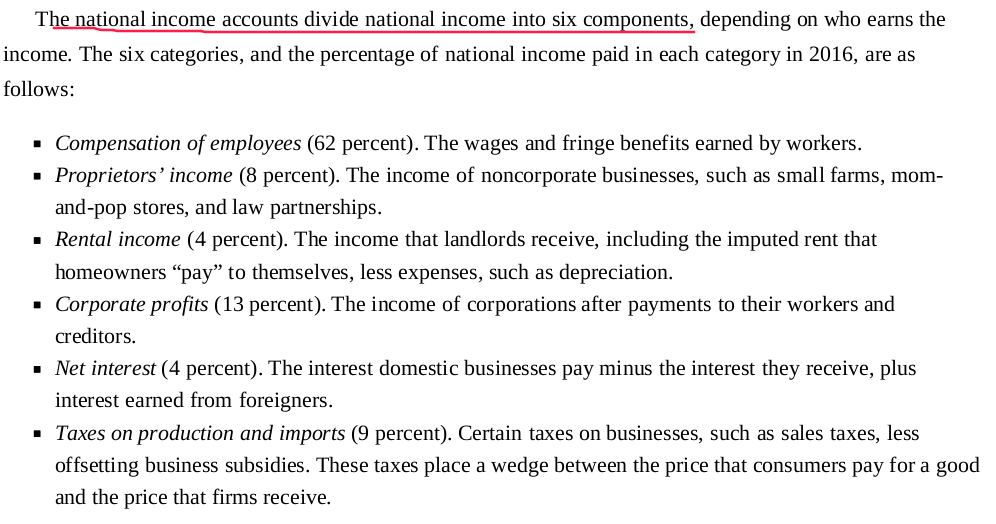
\includegraphics[scale =.5 ]  {figures/six_components_of_national_income.png}}
\end{figure}


\subsubsection{Personal Income}
A series of adjustments take us from national income to personal income, the amount of 
income that households and noncorporate businesses receive.

\begin{figure}[H]
\center{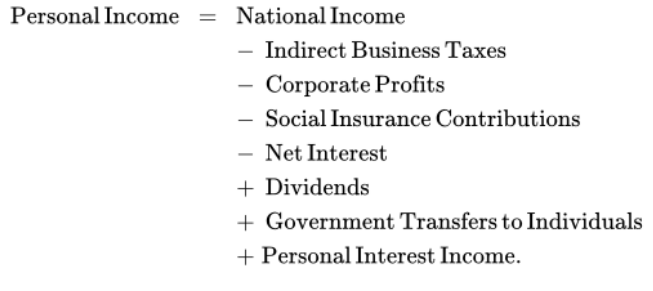
\includegraphics[scale =.5 ]  {figures/personal_income.png}}
\end{figure}

Indirect Business Taxes: we subtract taxes on production and imports because these taxes
never enter anyone’s income.



{\textbf {Further}}, if we subtract personal taxes from personal income, we obtain
{\textbf {disposable personal income (DPI)}}.

\begin{equation*}
		DPI = PI - tax
\end{equation*}

\noindent\fbox{%
\parbox{\textwidth}{%
We are interested in {\textbf {disposable personal income}} because it is the amount 
households and noncorporate businesses have available to spend after satisfying their
tax obligations to the government.
}%
}\\




\subsection{Seasonal Adjustment}
Economists are interested in studying the quarter-to-quarter fluctuations. It is not 
surprising that real GDP follows a seasonal cycle.
When economists study fluctuations in real GDP and other economic variables,
they often want to eliminate the portion of fluctuations due to predictable seasonal 
changes. You will find that most of the economic statistics reported are seasonally 
adjusted.




\subsection{CPI: Measuring the cost of living}
The most commonly used measure of the level of prices is the consumer price index (CPI).
The Bureau of Labor Statistics (BLS) has the job of computing the CPI.

{\textbf {CPI turns the prices of many goods and services into a single index measuring
the overall level of prices.}}

The CPI is the price of this basket of goods and services relative to the price of 
the same basket in some base year.

{\textbf {Example:}} consumer buy 5 apples and 2 oranges, base year is 2017.

\begin{figure}[H]
\center{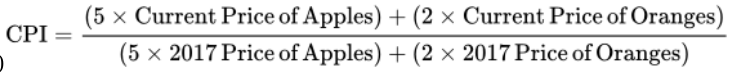
\includegraphics[scale =.6 ]  {figures/cpi_formula.png}}
\end{figure}

The index tells us how much it costs now to buy five apples and two
oranges relative to how much it cost to buy the same basket of fruit in 2017.

Other than CPI, we have other measurement of price, e.g., producer price index (PPI),
core inflation (measures the increase in price of a consumer basket that excludes 
food and energy products, because these two exhibit substantial short-run volatility
in price).




\noindent\fbox{%
\parbox{\textwidth}{%
{\textbf {Problems of CPI}}

1. Substitution Bias: does not consider the SE from price changing.\\
2. Ignorance of benefit from new goods. When a new good is introduced into the mkt,
consumers are better off because they have more products from which to choose. 
The introduction of new goods increases the real value of the dollar, but is not
reflected in a lower CPI.\\
3. Unmeasured change in quality.

}%
}\\




\subsubsection{CPI vs. GDP deflator}

1.\\
GDP deflator measures the prices of {\textbf {all}} goods and services. \\
CPI: prices of goods and services bought by {\textbf {consumers}}.\\


2.\\
GDP deflator includes only goods produced {\textbf {domestically}}.(no import)\\
CPI includes those import goods bought by consumers.
For example, an increase in the price of Toyotas made in Japan and sold in this 
country affects the CPI


3.\\
CPI assigns fixed weights to the prices of different goods because CPI is computed using
a fixed basket of goods.\\
GDP deflator assigns changing weights because the composition of GDP changes over time.


\noindent\fbox{%
\parbox{\textwidth}{%
{\textbf {Laspeyres vs. Paasche index}}\\
Laspeyres index: price index with a fixed basket of goods.\\
Paasche index: price index with a changing basket of goods.

Laspeyres index will overstate the increase of cost of living because it does not
consider the substitution effect (Q is fixed) due to the change in price.

Paasche index will understate the increase because even though it considers the SE, 
it does not reflect the reduction in consumer's welfare due to the substitution.
}%
}\\

{\textbf {CPI is a Laspeyres index, it overstate the impact of price changing.}}\\
{\textbf {GDP deflator is a Paasche index, it understate the impact.}}


\subsubsection{Another measurement of inflation other than CPI and GDP deflator}
The implicit price deflator for Personal Consmption Expenditures (PCE).

PCE deflator is calculated like the GDP deflator but it is only based on consumption
component.
\begin{equation*}
\text{ PCE deflator } = \frac{\text{ Nominal consumer spending }}{\text{ Real 
consumer spending}}
\end{equation*}


{\textbf {Luckily, the differences among these measures of inflation are usually
small in practice.}}

\begin{figure}[H]
\center{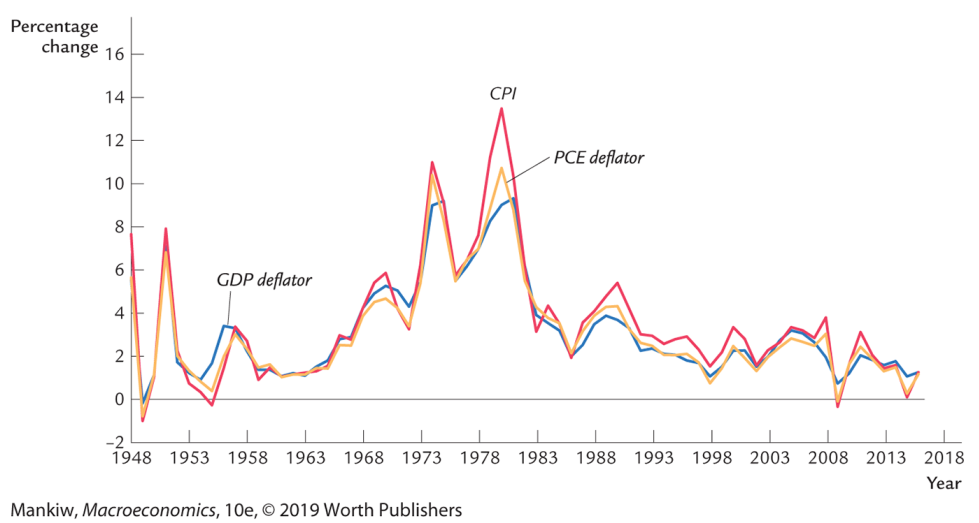
\includegraphics[scale =.5 ]  {figures/CPI_GDP_PCE.png}}
\end{figure}








\subsection{The Unemployment Rate}
Three status:
Employed, Unemployed, Not in the labor force.

A person who wants a job but has given up looking is counted as Not in the labor force.


\begin{align*}
\text{ Labor force } &= \text{ Employed }  + \text{ Unemployed }\\
\text{ Unemployment rate } &= \frac{\text{ Unemployed }}{\text{ Labor Force }} \times 
100\\
\text{ Labor force participation rate } &= 
\frac{\text{ Labor force }}{\text{ Adult population }} \times 100
\end{align*}


The BLS conducts two surveys of labor-market conditions, it produces two measures of 
total employment. 

1. From the household survey, it obtains an estimate of the number of people who say they
are working. 

2. From the establishment survey, it obtains an estimate of the number of workers firms 
have on their payrolls.


The data of these two are expected to be identical, but they are not.\\
Reasons:\\
1. Two surveys measure different things. Self-employed person is counted as employed in 
the household survey, but not in the establishment survey.\\
2. Two surveys are imperfect. It takes some time for new firms to be included in the
establishment survey. Also, the BLS can use incorrect estimates of the size of population
because of the changes in the rate of immigration, both legal and illegal.







\section{National Income}


\begin{figure}[H]
\center{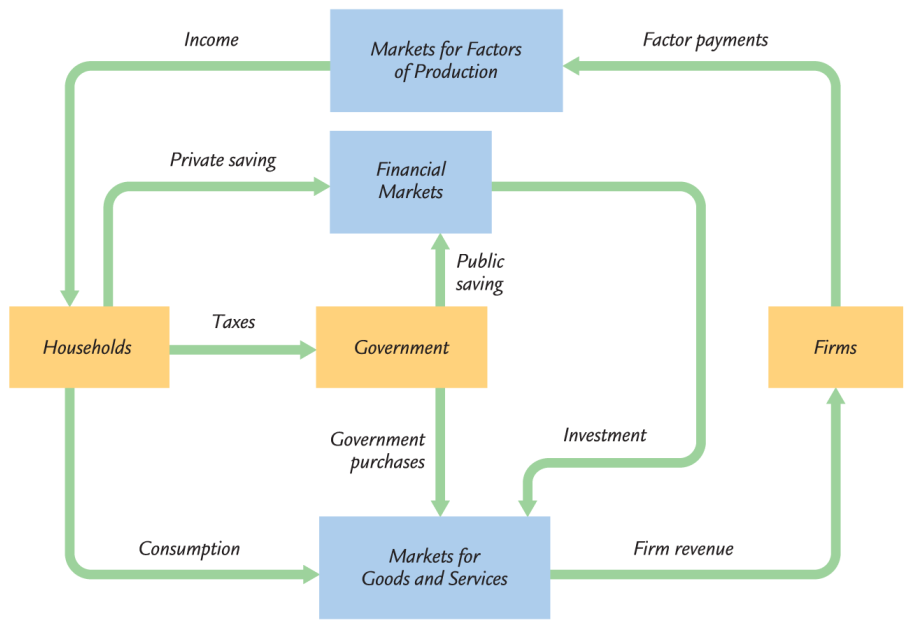
\includegraphics[scale =.5 ]  {figures/circular_flow_nation_economy.png}}
\end{figure}

Any excess of tax revenue over government spending is called {\textbf {public savings}}.
It can be positive or negative.


\subsection{Production}

\subsubsection{Production function}
\begin{equation*}
Y = F(K, L)
\end{equation*}

Many production functions are constant return to scale.
\begin{equation*}
\lambda Y = F(\lambda K, \lambda L)
\end{equation*}

\subsubsection{Classical and neoclassical theory}
They explained how national income is divided among the factors.

{\textbf {Classical:}}\\
Prices adjust to balance supply and demand.

{\textbf {Neoclassical:}}\\
Demand for each factor depends on the marginal productivity of that factor.


\subsubsection{Decision making for a competitive firms}
{\textbf {Assumptions:}}\\
Because there are many firms in the market,\\
1. Firms cannot affect the price of goods.\\
2. Firms cannot influence the wages.\\
3. Households rent their capital to firms.\\


{\textbf {Labor:}}

\begin{equation*}
\Pi = pF(K,L) - wL - rK
\end{equation*}
Differentiate $ \Pi $ wrt L,
\begin{align*}
p  \times MPL  - w &= 0\\
MPL &= \frac{w}{p}, \quad \text{ real wage }
\end{align*}

For any given real wage, the firm hires up to the point at which the MPL equals the 
real wage. Hence, the MPL schedule is also the firm’s labor demand curve.

\begin{figure}[H]
\center{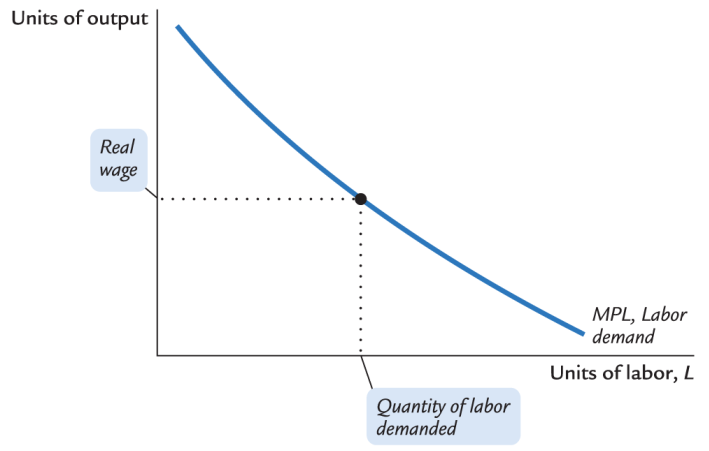
\includegraphics[scale =.5 ]  {figures/MPL.png}}
\end{figure}



{\textbf {Capital:}}

\begin{equation*}
\Pi = pF(K,L) - wL - rK
\end{equation*}
Differentiate $ \Pi $ wrt K,
\begin{align*}
p  \times MPK  - r &= 0\\
MPL &= \frac{r}{p}, \quad \text{ real rental price }
\end{align*}

{\textbf {The firm demands each factor of production until that factor’s marginal 
product equals its real factor price.}}


\subsection{The division of National Income}

Recall the real wages paid to labor are $ MPL  \times L $, and the real return paid to
capital owners is $ MPK  \times K $.

{\textbf {Economic profit}}:

The income that {\textbf {remains}} after the firms have paid the factors is the 
{\textbf {economic profit}} of the owners of the {\textbf {firms}}:
\begin{equation*}
\text{ Econ Profit } = Y/p - (MPL  \times L) - (MPK  \times K)
\end{equation*}

Note, $ Y = p F(K,L) $.

We can rewrite the Econ Profit equation to examine the distribution of income:
\begin{equation*}
Y = (MPL  \times L) + (MPK  \times K) + \text{ Econ Profit }
\end{equation*}

Total income is divided among the return to labor, the return to capital, and economic 
profit.

{\textbf {NOTE:}} According to the Euler's theorem, if the production function is
constant return to scale, then {\textbf {the economic profit must be ZERO}},
\begin{equation*}
F(K,L) = MPK  \times r + MPL  \times L
\end{equation*}


In the real world, however, most firms own rather than rent the capital they use. The
econ profit and the return to capital are often lumped together. We call this 
accounting profit,
\begin{equation*}
\text{ Accounting profit } = \text{ Econ profit } + MPK  \times K.
\end{equation*}

\subsubsection{Cobb-Douglas}

\begin{equation*}
Y = AK^{\alpha}L^{1 - \alpha}
\end{equation*}

\begin{align*}
MPK &= \alpha AK^{\alpha - 1}L^{1 - \alpha} = \frac{\alpha Y}{K}\\
MPL &= (1 - \alpha)AK^{\alpha}L^{ - \alpha} = \frac{(1 - \alpha)Y}{L}
\end{align*}
where $ Y/K $ is the {\textbf {average capital productivity}}, $ Y/L $ is the 
{\textbf {average labor productivity}}.


{\textbf {If factors earn their marginal products, then parameter $ \alpha $ tells us
how much income goes to labor and how much goes to capital.}}\\
The total amount paid to labors are $ MPL  \times L = (1 - \alpha)Y $,\\
The total amount paid to capital are $ MPK  \times K = \alpha Y $,\\
{\textbf {NOTE:}} The shares depend ONLY on $ \alpha $, not on the amounts of K and L, or
on the state of technology $ A $.


\subsection{What determines the demand for goods and services}

\begin{equation*}
Y = C + I + G + NX
\end{equation*}

Suppose there is a closed economy, i.e., $ NX = 0 $. Write down the national income 
accounts identity.

\begin{equation*}
Y = C + I + G
\end{equation*}

\subsubsection{Consumption}
The disposable income (after tax income) is $ Y - T $. Therefore, the consumption is
a function of the disposable income,
\begin{equation*}
C = C(Y - T)
\end{equation*}

The {\textbf {Marginal Propensity to Consume (MPC)}} is the amount by which consumption
changes when disposable income increases by one dollar. ($ MPC \in [0,1] $)
MPC is the slope of the consumption function.

\begin{figure}[H]
\center{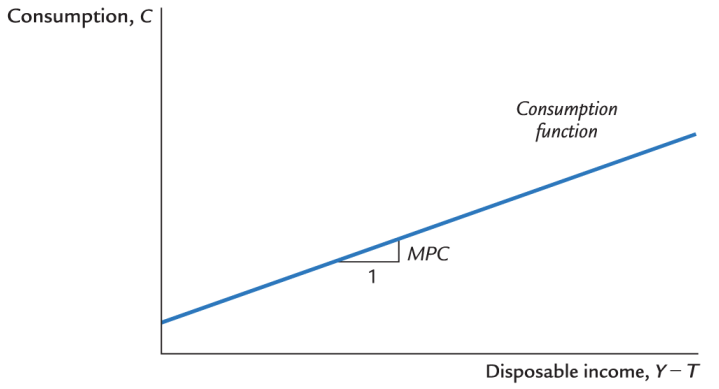
\includegraphics[scale =.5 ]  {figures/MPC.png}}
\end{figure}

\subsubsection{Investment}
The Q of investment goods demanded depends on the {\textbf {interest rate}}, which
measures the cost of the funds used to finance investment. The return (the revenue
from increased future production of goods and services) must exceed its cost (the 
payments for borrowed funds) if an investment project is profitable.

If the interest rate rises, investment falls.\\

{\textbf {Nominal Interest rate vs. Real Interest rate}}\\
Economists distinguish between the nominal interest rate and the real interest rate.
\begin{equation*}
\text{ Nominal interest rate } = \text{ Real Interest rate } + \text{ Inflation rate }
\end{equation*}

{\textbf {The real interest rate, $ r $, measures the true cost of borrowing and, 
thus, determines the quantity of investment.}}
\begin{equation*}
I = I(r)
\end{equation*}


\begin{figure}[H]
\center{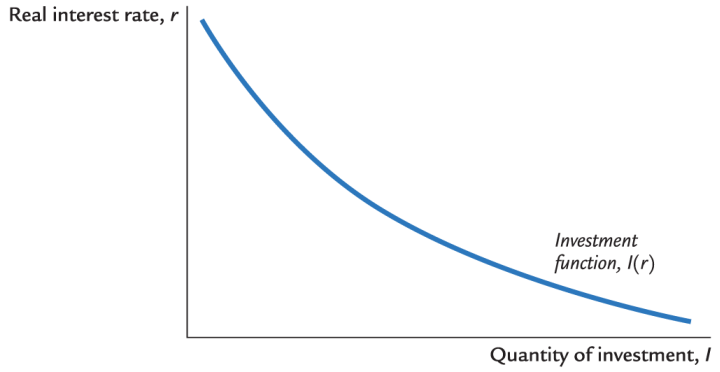
\includegraphics[scale =.5 ]  {figures/investment.png}}
\end{figure}

There are many interest rate in the real world. They are different in three ways:\\
1. Term. Long term and short term interest rate. Long term's are usually, but not always,
higher than short term interest rate.

2. Credit risk. The higher the perceived probability of default, the higher the interest
rate. Government has the lowest credit risk, therefore government bonds tend to pay
a low interest rate.

3. Tax treatment. The interest on different types of bonds is taxed differently. Most important, when state and local governments issue bonds, called municipal bonds, the holders of the bonds do not pay federal income
tax on the interest income. Because of this tax advantage, municipal bonds pay a lower interest rate.



\subsubsection{Government Purchases}
Two types of government spending: government purchases and government transfer.

Gov't purchases: guns, missile, roads, library, etc. They are $ G $.\\
Gov't transfer: transfer payments to households, e.g., public assistance for the poor.
Transfer payments are not made in exchange for some of the economy's output of goods
and services. Therefore, {\textbf {they are not included in $ G $}}.


Now we can redefine $ T $. 
\begin{equation*}
T = \text{ tax } - \text{ transfer }
\end{equation*}
So the disposable income, $ Y - T $, includes both the negative impact of taxes and 
the positive impact of transfer payments.


The government has a balanced budget: $ G = T $.\\
The government has a budget deficit: $ G > T $.\\
The government has a budget surplus: $ G < T $.\\

{\textbf {Assumptions:}}
Endogenous variables: C, I, r\\
Exogenous variables: G



\subsection{Market Equilibrium}

{\textbf {Demand side:}}
\begin{align*}
Y &= C + I + G\\
C &= C(Y - T)\\
I &= I(r)\\
G &=  \overline{G}\\
T &=  \overline{T}
\end{align*}


{\textbf {Supply side:}}
\begin{equation*}
Y = F(K,L)
\end{equation*}
If we assume $ K $ and $ L $ are fixed, we can write
\begin{equation*}
Y =  \overline{Y} = F( \overline{K},  \overline{L})
\end{equation*}

{\textbf {Combine D and S:}}
\begin{align*}
\overline{Y} = F( \overline{K},  \overline{L}) &= C(Y - T) + I(r) + G\\
\overline{Y} &= C( \overline{Y} -  \overline{T}) + I(r) +  \overline{G}
\end{align*}

The LHS is the supply of outputs, the RHS is the demand of outputs.

Only investment, $ I $, is changed. 
If $ r $ goes up, $ I $ goes down, the demand for goods and services is less than the
supply for them.\\
If $ r $ goes down, $ I $ goes up, the demand for goods and services is greater than the
supply for them.

At the equilibrium, S = D.

Then, how does the interest rate get to the level that balances the supply and demand
for goods and service? See next section.


\subsubsection{Equilibrium in the financial market}
Rewrite the national income account identity:
\begin{equation*}
Y - C - G = I
\end{equation*}
LHS is savings, $ S $.
\begin{equation*}
S = Y - C - G = I
\end{equation*}

We can further split this into two parts:
\begin{equation*}
S = (Y - T - C) + (T - G) = I
\end{equation*}
where $ (Y - T - C) $ represents {\textbf {private saving}}, and $ (T - G) $ represents
{\textbf {public saving.}}

It says that the flows into the financial markets (private and public savings) 
{\textbf {must}} balance the flows out of the financial markets (investment).

Further, we can write,
\begin{align*}
\overline{Y} - C( \overline{Y} -  \overline{T}) -  \overline{G} &= I(r)\\
 \overline{S} &= I(r)
\end{align*}

Because we assume Y is fixed by K and L, LHS is fixed. And we can draw the graph,

\begin{figure}[H]
\center{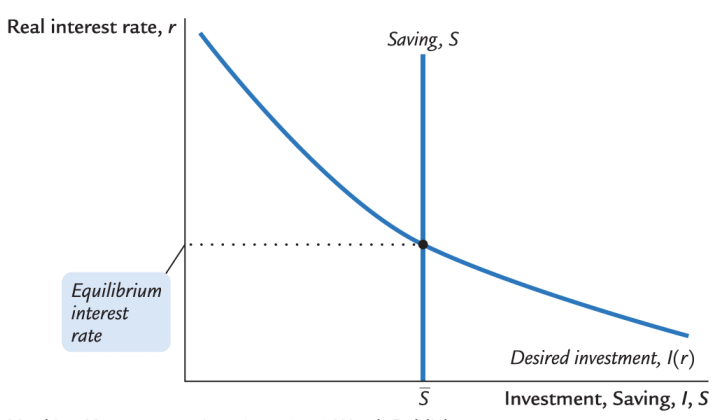
\includegraphics[scale =.5 ]  {figures/saving_investment.png}}
\end{figure}

Here saving function is a vertical line because it does not depends on interest rate 
(We will relax this later on).

We can interpret this from Supply and Demand perspective. The product is {\textbf {
loanable funds}}, price is the real interest rate.\\
Supply (saving) side, HHs lend their savings or deposit to banks. \\
Demand (investment) side, investors borrow from the public by selling bonds or 
by borrowing from banks.

The interest rate adjust until Q of Demand equals Q of Supply. If $ r $ is too low,
Q of D $ > $ Q of S, more people want to borrow money. So $ r $ will rise, vice versa.



\subsubsection{Changes in Saving: The effects of Fiscal Policy}

Two factors affect savings: G and T


When govt changes its spending or the level of taxes, it affects the demand for the
economy's output of goods and services and alters national savings, investment, and
the interest rate.

{\textbf {Factor 1: Change in government purchases (G)}}

Recall
\begin{align*}
S = Y - C - G &= I\\
S = (Y - T - C) + (T - G) &= I
\end{align*}

C is a function of $ Y - T $, not affected by G. Y is not affected by G. So, if G 
goes up, saving goes down (public saving), therefore $ I $ goes down.

If G goes up, then S goes down, $ r $ goes up, $ I $ goes down.
\begin{figure}[H]
\center{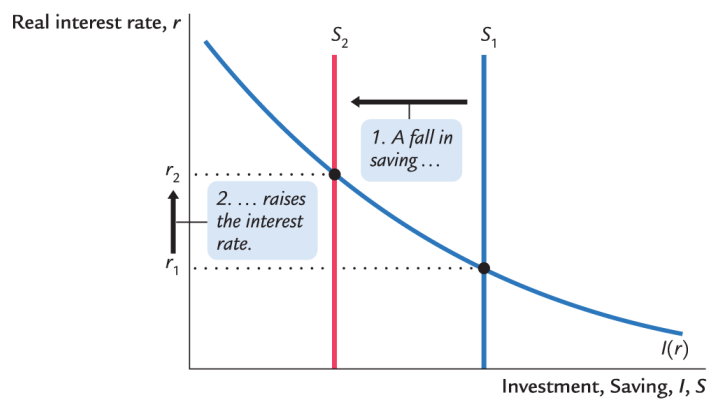
\includegraphics[scale =.5 ]  {figures/change_in_G.png}}
\end{figure}




{\textbf {Factor 2: Change in taxes (T)}}

Recall,
\begin{equation*}
S = Y - C - G = I
\end{equation*}
where $ C = C(Y - T) $.\\
If $ T $ goes down, $ C $ goes up, $ S $ goes down, $ I $ goes down.

The change of consumption, $ \Delta C $, depends on MPC and $ \Delta T $.
\begin{equation*}
\Delta C = MPC  \times \Delta T
\end{equation*}
Remember, MPC is the slope of consumption function.

The reduction in savings shift the supply to the left, $ r $ goes up, $ I $ goes down.



\subsubsection{Changes in Investment Demand}


Demand shifter: technology innovation, government policy (increase/decrease tax)

Innovation of new technology requires large investment, it increase the demand of 
investment (shift the demand curve up).

Government can increase personal tax to provide tax cuts for those firms who invest
in new capital. It makes more investment projects profitable, shift the demand of 
investment up.

While Saving is fixed, if demand goes up, $ r $ goes up, $ I $ not change.
\begin{figure}[H]
\center{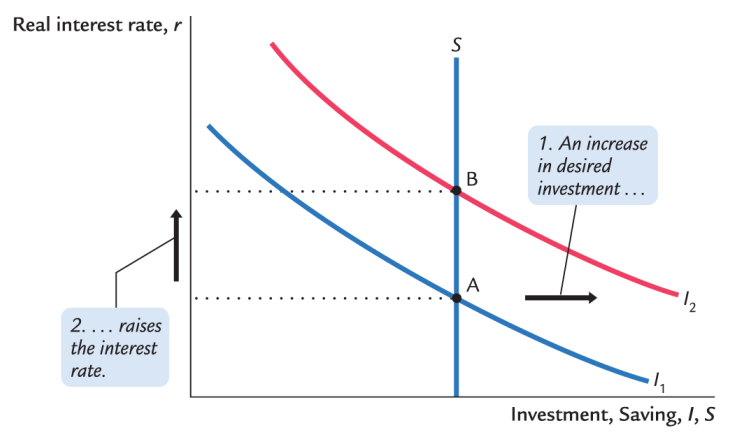
\includegraphics[scale =.5 ]  {figures/change_in_demand_investment.png}}
\end{figure}


If we relax the fixed saving assumption, allowing change in consumption (depends on
the interest rate), we have an upward Saving (supply) curve.\\
If demand goes up, $ r $ goes up , $ I $ goes up.\\
The increase in $ r $ will reduce the consumption, frees resources for investment.

\begin{figure}[H]
\center{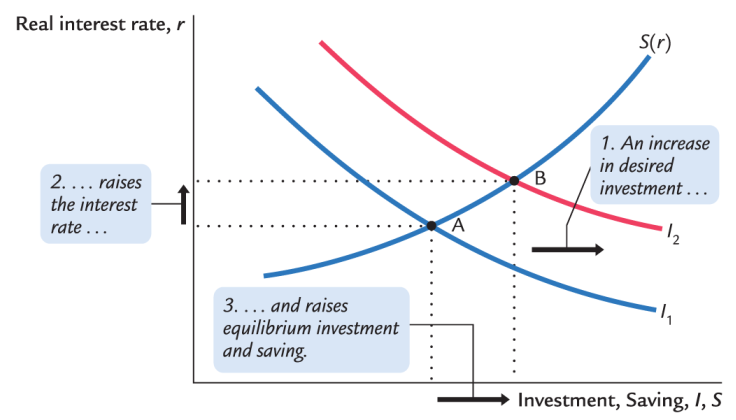
\includegraphics[scale =.5 ]  {figures/change_in_demand_upward_supply.png}}
\end{figure}




\subsection{Conclusion}
The model relies on {\textbf {classical}} assumption that prices adjust to equilibrate
supply and demand, e.g., factor prices equilibrate factor mkts, $ r $ equilibrate the
supply and demand of investment.
The model incorporates all the interactions illustrated in the circular flow, it is
sometimes called a {\textbf {general equilibrium model}}.




\section{The monetary system}

The two arms of macroeconomic policy are monetary and fiscal policy.\\
{\textbf {Fiscal policy}} encompasses the government’s decisions about spending and 
taxation, as we saw in the previous chapter. Elected representatives make fiscal policy,
e.g., U.S. Congress, British Parliament.\\
{\textbf {Monetary policy}} refers to decisions about the nation’s system of coin,
currency, and banking. The government's control over the money supply. Central Banks 
make monetary policy. CB is set up by the elected representatives, but operates 
independently.


\subsection{Money}
\subsubsection{Functions of money}
1. store of value\\
2. unit of account\\
3. medium of exchange


\subsubsection{Types of money}
Fiat money: Money without intrinsic value (it is established by government decree).\\
Commodity money: Money with intrinsic value, e.g., gold.



\subsection{Monetary policy}

Decisions about monetary policy are made by the Fed's Federal Open Market Committee (
FOMC). FOMC meets about every six weeks to discuss and set monetary policy.


\subsubsection{Methods of control on money supply}

1. Through open-market operations (Federal reserve): purchase and sell of government 
bonds. To increase money supply, Fed buys bonds from the public.\\
2. Behavior of households and banks (fractional-reserve banking).



\subsubsection{Measurement of quantity of money}
quantity of money = currency + demand deposits + funds in savings account

demand deposits: funds people hold in their checking account.

\begin{figure}[H]
\center{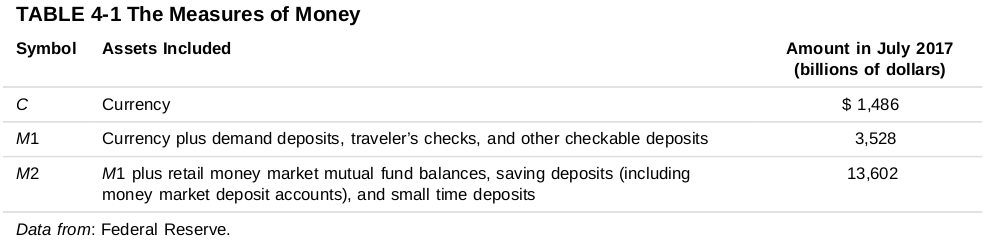
\includegraphics[scale =.6 ]  {figures/measures_of_money.png}}
\end{figure}

\noindent\fbox{%
\parbox{\textwidth}{%
Are credit cards and debit cards fit into monetary system?\\

Debit card links to bank account, gives users {\textbf {immediate}} access to deposit.
It is included in measures of the quantity of money.

Credit card, however, is {\textbf {NOT}} included in the measures of the quantity of
money because credit card is a deferring payment. You need to repay the funds from your
bank account later on.
}%
}\\




We begin with the relationship between money supply (M), currency (C), and demand
deposits (D):
\begin{equation*}
M = C + D
\end{equation*}





{\textbf {Fully-reserve banking:}}

The deposits that banks have received but have not lent out are called 
{\textbf {reserves}}.
Some reserves are held in the vaults of local banks throughout the country,
but most are held at a central bank, such as the Federal Reserve.

If household deposit \$1000 in bank account, and the bank hold this as reserve, it
is called fully-reserve banking.

\begin{figure}[H]
\center{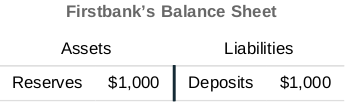
\includegraphics[scale =.7 ]  {figures/fully_reserve_banking.png}}
\end{figure}

Recall $ M = C + D $, HH deposit \$1000 currency (C) to demand deposit (D), money
supply (M) is not change.\\




{\textbf {Fractional-reserve banking:}}

Banks can also lend out part of the reserve earning interest, only hold part of the 
reserve, this is called fractional-reserve banking.


\begin{figure}[H]
\center{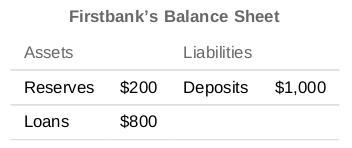
\includegraphics[scale =.8 ]  {figures/fractional_reserve_banking.png}}
\end{figure}

{\textbf {Notice:}} bank increase the money supply by \$800 when it makes this loan.
Before the loan, the money supply = 1000 = deposits. After the loan is made, 
the money supply = 1000 + 800 = 1800, now borrower holds 800 in currency.

Before:
\begin{equation*}
		1000(M) = 0(C) + 1000(D)
\end{equation*}
After:
\begin{equation*}
		1800(M) = 800(C) + 1000(D)
\end{equation*}

Thus, {\textbf {in a system of fractional-reserve banking, banks create money.}}





Suppose we have another bank that receives the deposit of this \$800, and then it
holds 20\%(160) as reserve and lend out the rest (640), the balance sheet would be,

\begin{figure}[H]
\center{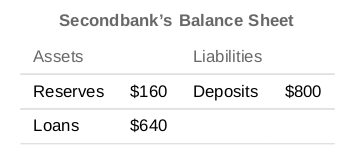
\includegraphics[scale =.7 ]  {figures/second_bank.png}}
\end{figure}

Then the third bank receive this 640, hold 20\% and lend out the rest,

\begin{figure}[H]
\center{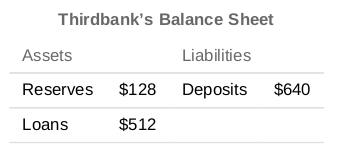
\includegraphics[scale =.7 ]  {figures/third_bank.png}}
\end{figure}

Keep iterating this, the banks are keep creating money. {\textbf {But their is an
upper bound for this augmentation}}. Define the {\textbf {reserve-deposit ratio}} as 
$ rr $,
\begin{align*}
\text{ Original deposit } &= 1000\\
\text{ first bank lending }  &= (1 - rr) \times 1000\\
\text{ second bank lending }  &= (1 - rr)^{2} \times 1000\\
\text{ third bank lending }  &= (1 - rr)^{2} \times 1000\\
...
\end{align*}
The total money supply would be:
\begin{align*}
M &= \left[ 1 + (1 - rr) + (1 - rr)^{2} + (1 - rr)^{3} + ... \right]  \times 1000\\
	&= \frac{1 - (1 - rr)^{n}}{1 - (1 - rr)}  \times 1000\\
	&= \frac{1}{rr} \times 1000
\end{align*}

Each \$1 of reserves generates \$$ (\frac{1}{rr}) $ of money. In our case, $ rr = 0.2 $



\noindent\fbox{%
\parbox{\textwidth}{%
Note, although the system of fractional-reserve banking creates money, it DOES NOT
create wealth. Borrowers still need to repay the debt. {\textbf {Creation of money
by the banking system increases the economy's liquidity, not its wealth.}}
}%
}\\



\subsubsection{Bank capital, leverage, and capital requirements}



\begin{figure}[H]
\center{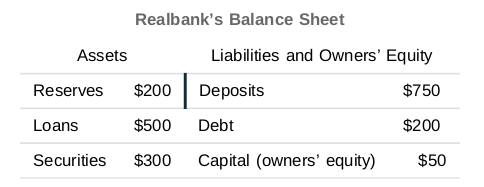
\includegraphics[scale =.7 ]  {figures/realbank_balance_sheet.png}}
\end{figure}

{\textbf {Leverage:}}\\
It is the use of borrowed money to supplement existing funds for purposes of 
investment.
\begin{equation*}
		\text{ leverage ratio } = \frac{\text{ total assets(LHS of the balance sheet) }}
		{\text{ the bank's capital (owner's equity) }}
\end{equation*}

In our case above, 
\begin{equation*}
\text{ leverage ratio } = \frac{200+500+300}{50} = \frac{1000}{50} = 20
\end{equation*}


High leverage ratio can be very risky. In our case, if th bank's assets fall in value
by just 5\%, the \$1000 is now \$950. Since the depositors and debt holders have the
legal right to be paid first, the owner's equity (\$50) falls to zero.

If the value of the assets fall more than 5\%, the bank capital goes below zero.
The bank is said to be {\textbf {insolvent}}.

This is why bank regulators require that banks hold sufficient capital (
{\textbf {capital requirement}}).



\subsubsection{How central banks influence the money supply}

{\textbf {A model of the money supply}}

We try to understand:
1. Fed's decision about how many dollars to create\\
2. Bank's decision about whether to hold deposits as reserve or to lend out\\
3. HH's decision about wheher to hold currency or demand deposits.


Three exogenous variables:\\
1. The monetary base (B):  sum of currency (C) held by the public and
the reserves (R) held by banks. {\textbf {$ B $ is directly controlled by the Fed.}}
$ B $ is also called the high-powered money.
\begin{equation*}
 B = C + R 
\end{equation*}
2. The reverse-deposit ratio (rr):
\begin{equation*}
rr = \frac{\text{ reverse }}{\text{ deposit }}
\end{equation*}
3. The currency-deposit ratio (cr): curency people hold as a fraction of their holdings
of demand deposits $ D $. {\textbf {It reflects the preference of HHs to the form
of money they wish to hold.}}
\begin{equation*}
cr = \frac{\text{ currency }}{\text{ deposit }}
\end{equation*}


Also, recall the definition of money supply,
\begin{equation*}
M = C + D
\end{equation*}

Now we can derive the {\textbf {money multiplier}}:
\begin{align*}
\frac{M}{B} &= \frac{C + D}{C + R}\\
 &= \frac{ \frac{C}{D} + 1}{ \frac{C}{D} + \frac{R}{D}}, \text{ devided by D }\\
 &= \frac{cr + 1}{cr + rr}\\
M &= \frac{cr + 1}{cr + rr} \times B
\end{align*}
where $ \frac{cr + 1}{cr + rr} $ is called the {\textbf {money multiplier}}. We can
write in this way
\begin{equation*}
M = m  \times B, \text{ where $ m $ is the multiplier }
\end{equation*}
\noindent\fbox{%
\parbox{\textwidth}{%
		It says each dollar of the monetary base (B) produces $ m $ dollars of money.\\
		Because the monetary base has a multiplied effect on the moeny supply, it is called
		{\textbf {high-powered money}}.\\
		Example:
		If B = 800, rr = 0.1, cr = 0.8,
		\begin{equation*}
		m = \frac{0.8 + 1}{0.8 + 0.1} = 2
		\end{equation*}
		\begin{equation*}
		M = 2  \times 800 = 1600
		\end{equation*}
}%
}\\

Change of M:\\
1. If B increase, M goes up.\\
2. Reduce in $ rr $ means, banks hold less reserve, lend out more (more loan),
create more money. So, reduce in $ rr $ will increase the multiplier (m) and the money 
supply (M).\\
3. Reduce in $ cr $ means, HHs hold less currency (deposit into banks), banks hold more
reserves, lend out more, multiplier goes up, $ M $ goes up.



\subsubsection{Monetary policy}

{\textbf {Ususally, the Fed controls the money supply indirectly through monetary
policy rather than directly change $ M $}}.

These tools can be classied into two groups: 1) those that influence the monetary base,
and 2) those that influence the reserve-deposit ratio ($ rr $) and thereby the 
monetary multiplier.\\

{\textbf {Change in monetary base ($ B = C + R $):}}\\
1. Fed can buy and sell bonds from/to the public. If Fed purchases bond from the
public, the public hold more currency, $ C $ goes up, $ B $ goes up, then money supply
($ m $) goes up, vice versa.

2. Fed can alter the monetary base and money supply by lending reserves to banks.
If banks borrow money from the Fed for whatever reason, reserve ($ R $) held by banks 
goes up, then monetary base ($ B $) goes up, and money supply ($ M $) goes up.\\
Banks need to pay interest to the Fed. If the Fed increase the interest rate (
discount rate), banks can borrow less, $ R $ goes down, $ M $ goes down.





















%\bibliographystyle{plainnat}
%\bibliography{my_bib}

\end{document}

